\chapter{Конструкторская часть}

\section{Схема алгоритма нахождения расстояния Левенштейна}

На рисунке \ref{img:levenstein} приведена схема нерекурсивного алгоритма поиска расстояния Левенштейна.

\begin{table}[h!]
	\centering
	\begin{tabular}{p{1\linewidth}}
		\centering
		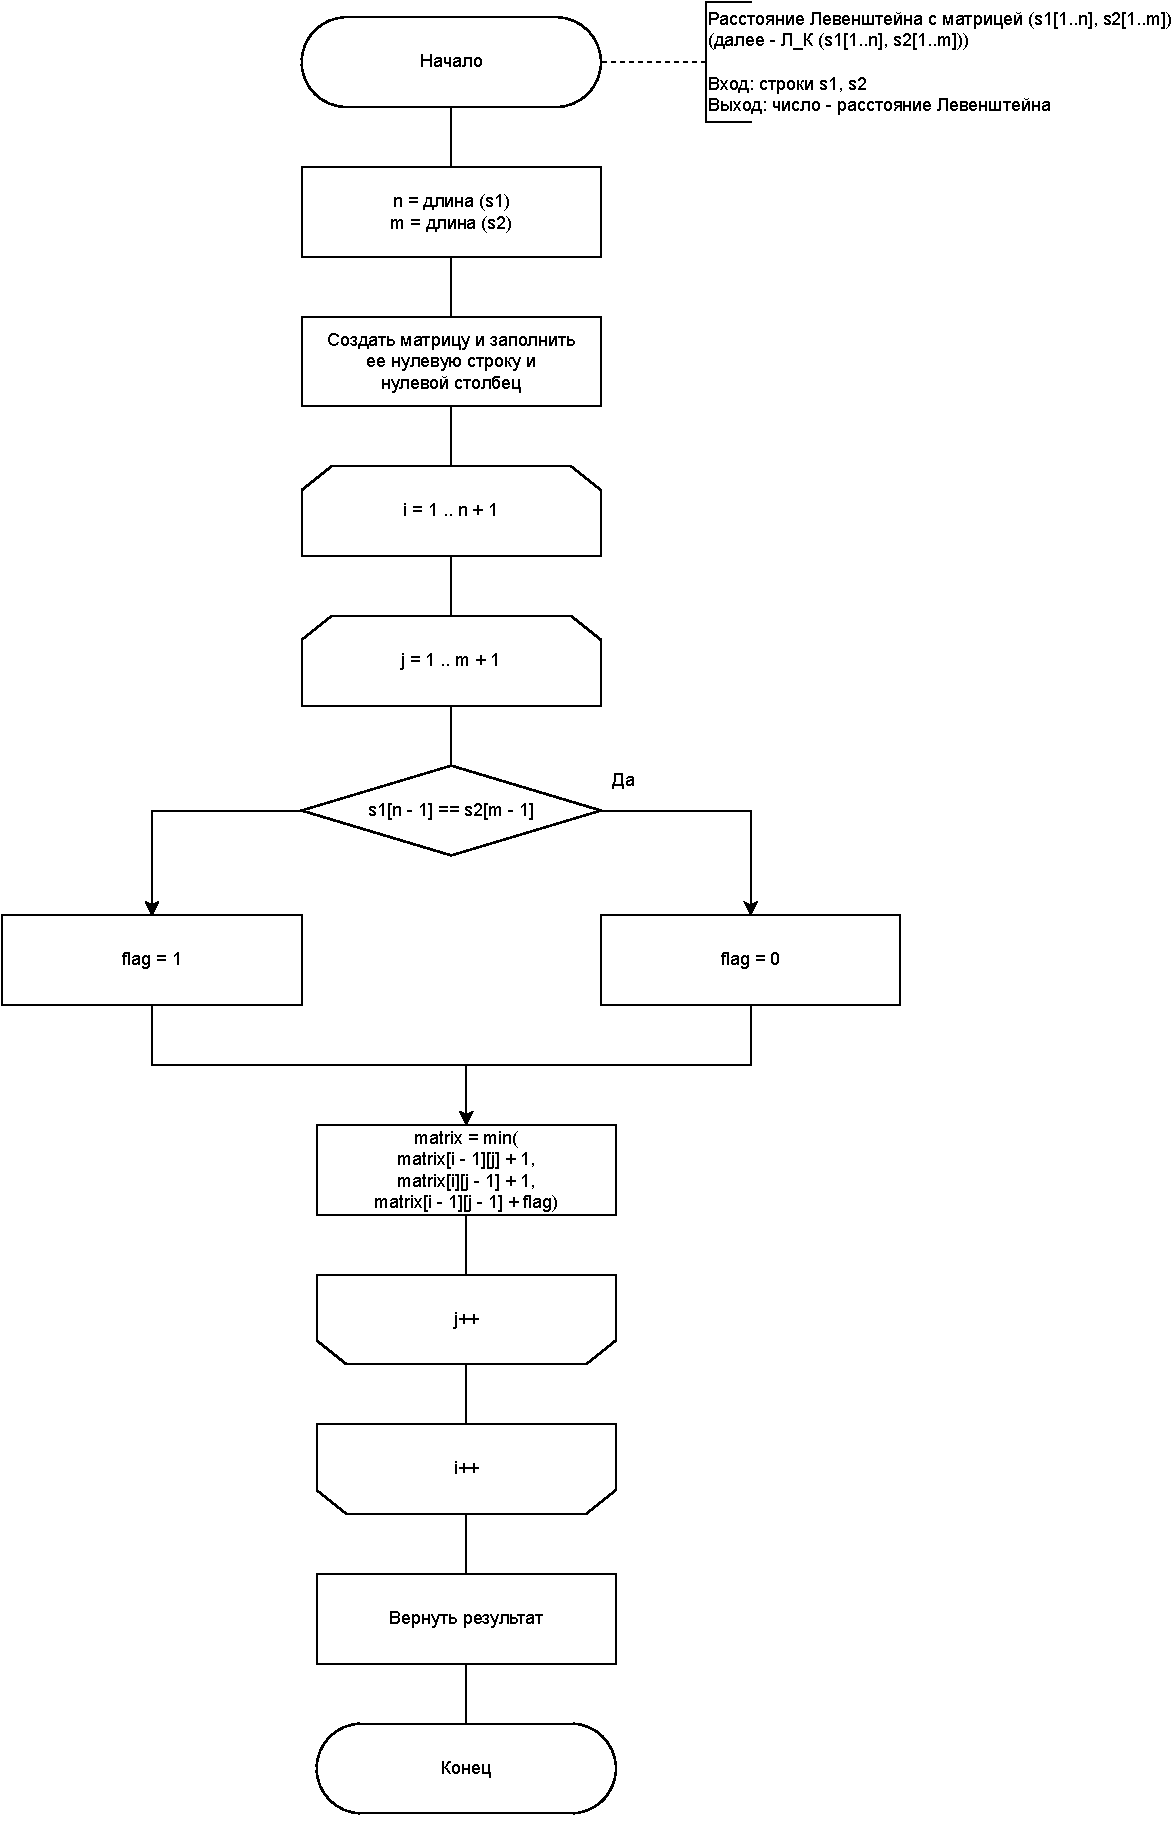
\includegraphics[width=0.8\linewidth]{include/lev.pdf}
		\captionof{figure}{Схема нерекурсивного алгоритма поиска расстояния Левенштейна}
		\label{img:levenstein}
	\end{tabular}
\end{table}

\section{Схемы алгоритмов нахождения расстояния Дамерау -- Левенштейна}

На рисунке \ref{img:damlev} приведена схема нерекурсивного алгоритма поиска расстояния Дамерау -- Левенштейна.

\begin{table}[h!]
	\centering
	\begin{tabular}{p{1\linewidth}}
		\centering
		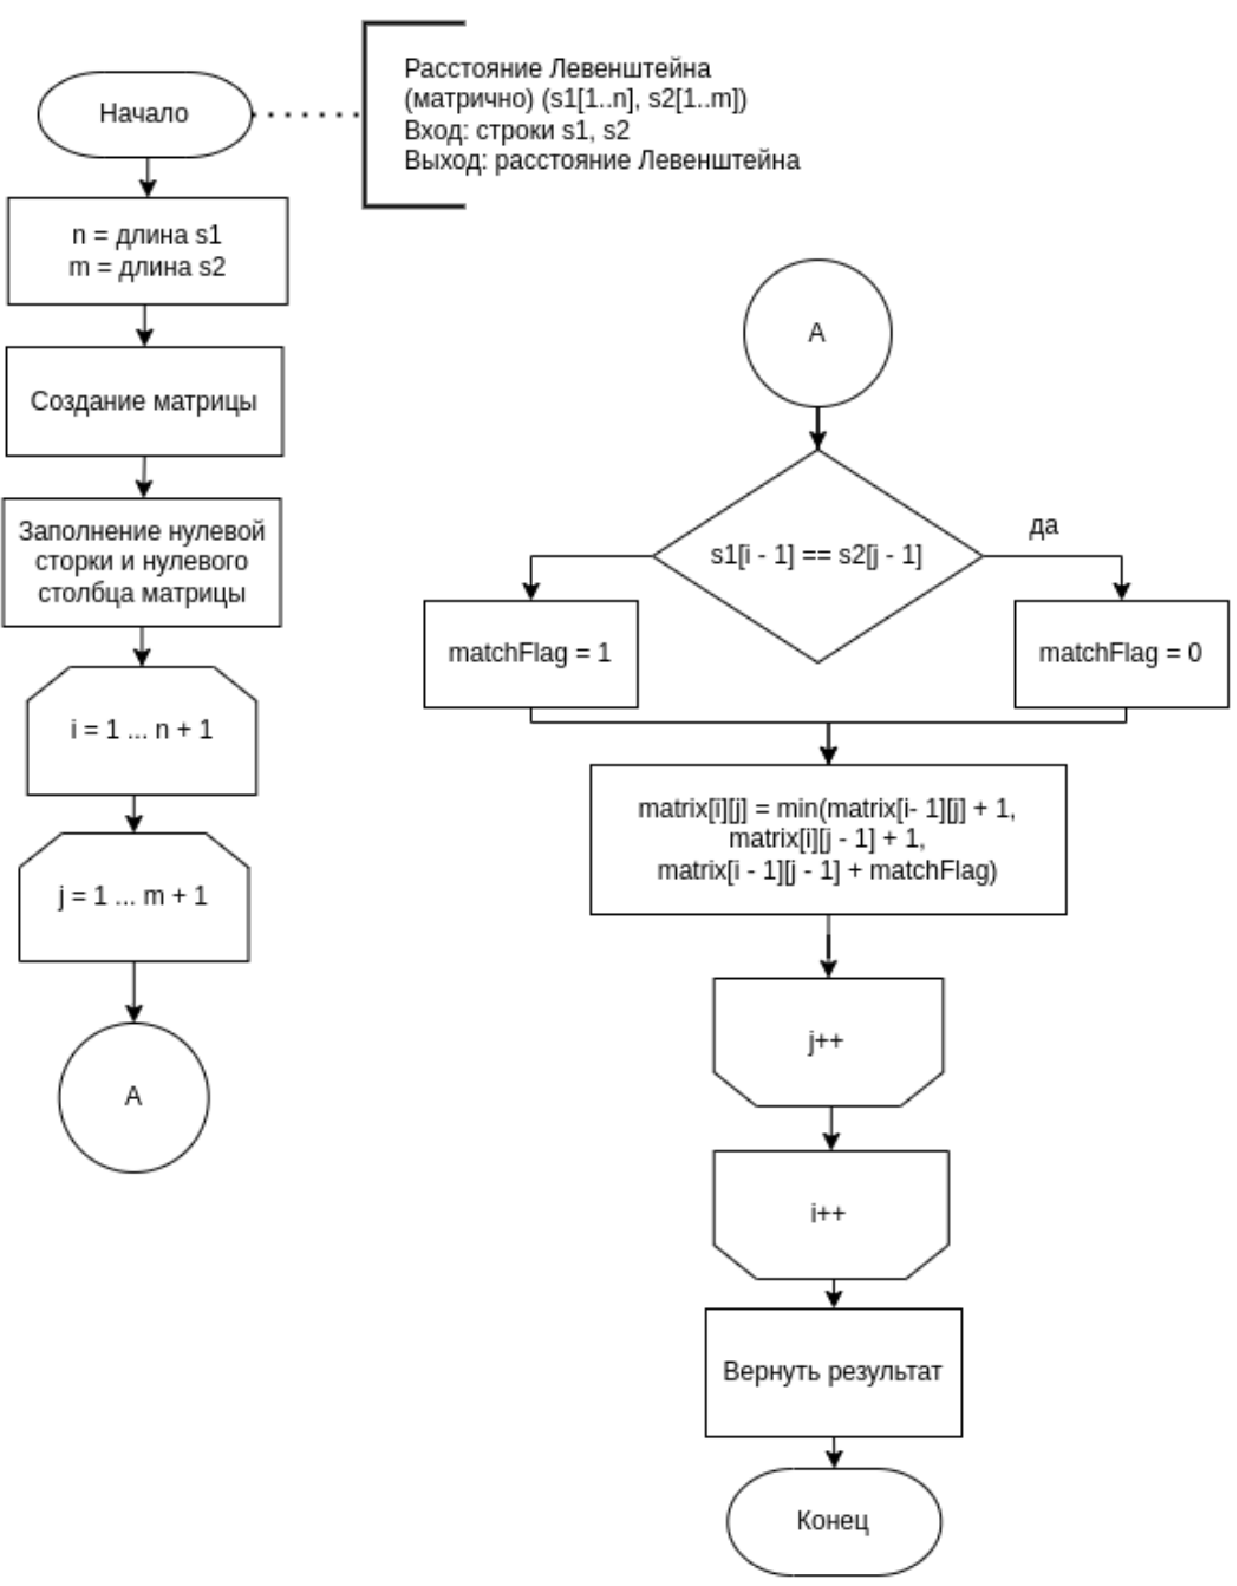
\includegraphics[width=0.8\linewidth]{include/damlev.pdf}
		\captionof{figure}{Схема нерекурсивного алгоритма поиска расстояния \\Дамерау -- Левенштейна}
		\label{img:damlev}
	\end{tabular}
\end{table}

Схема рекурсивного алгоритма поиска расстояния Дамерау -- Левенштейна представлена на рисунке \ref{img:recdamlev}.

\begin{table}[h!]
	\centering
	\begin{tabular}{p{1\linewidth}}
		\centering
		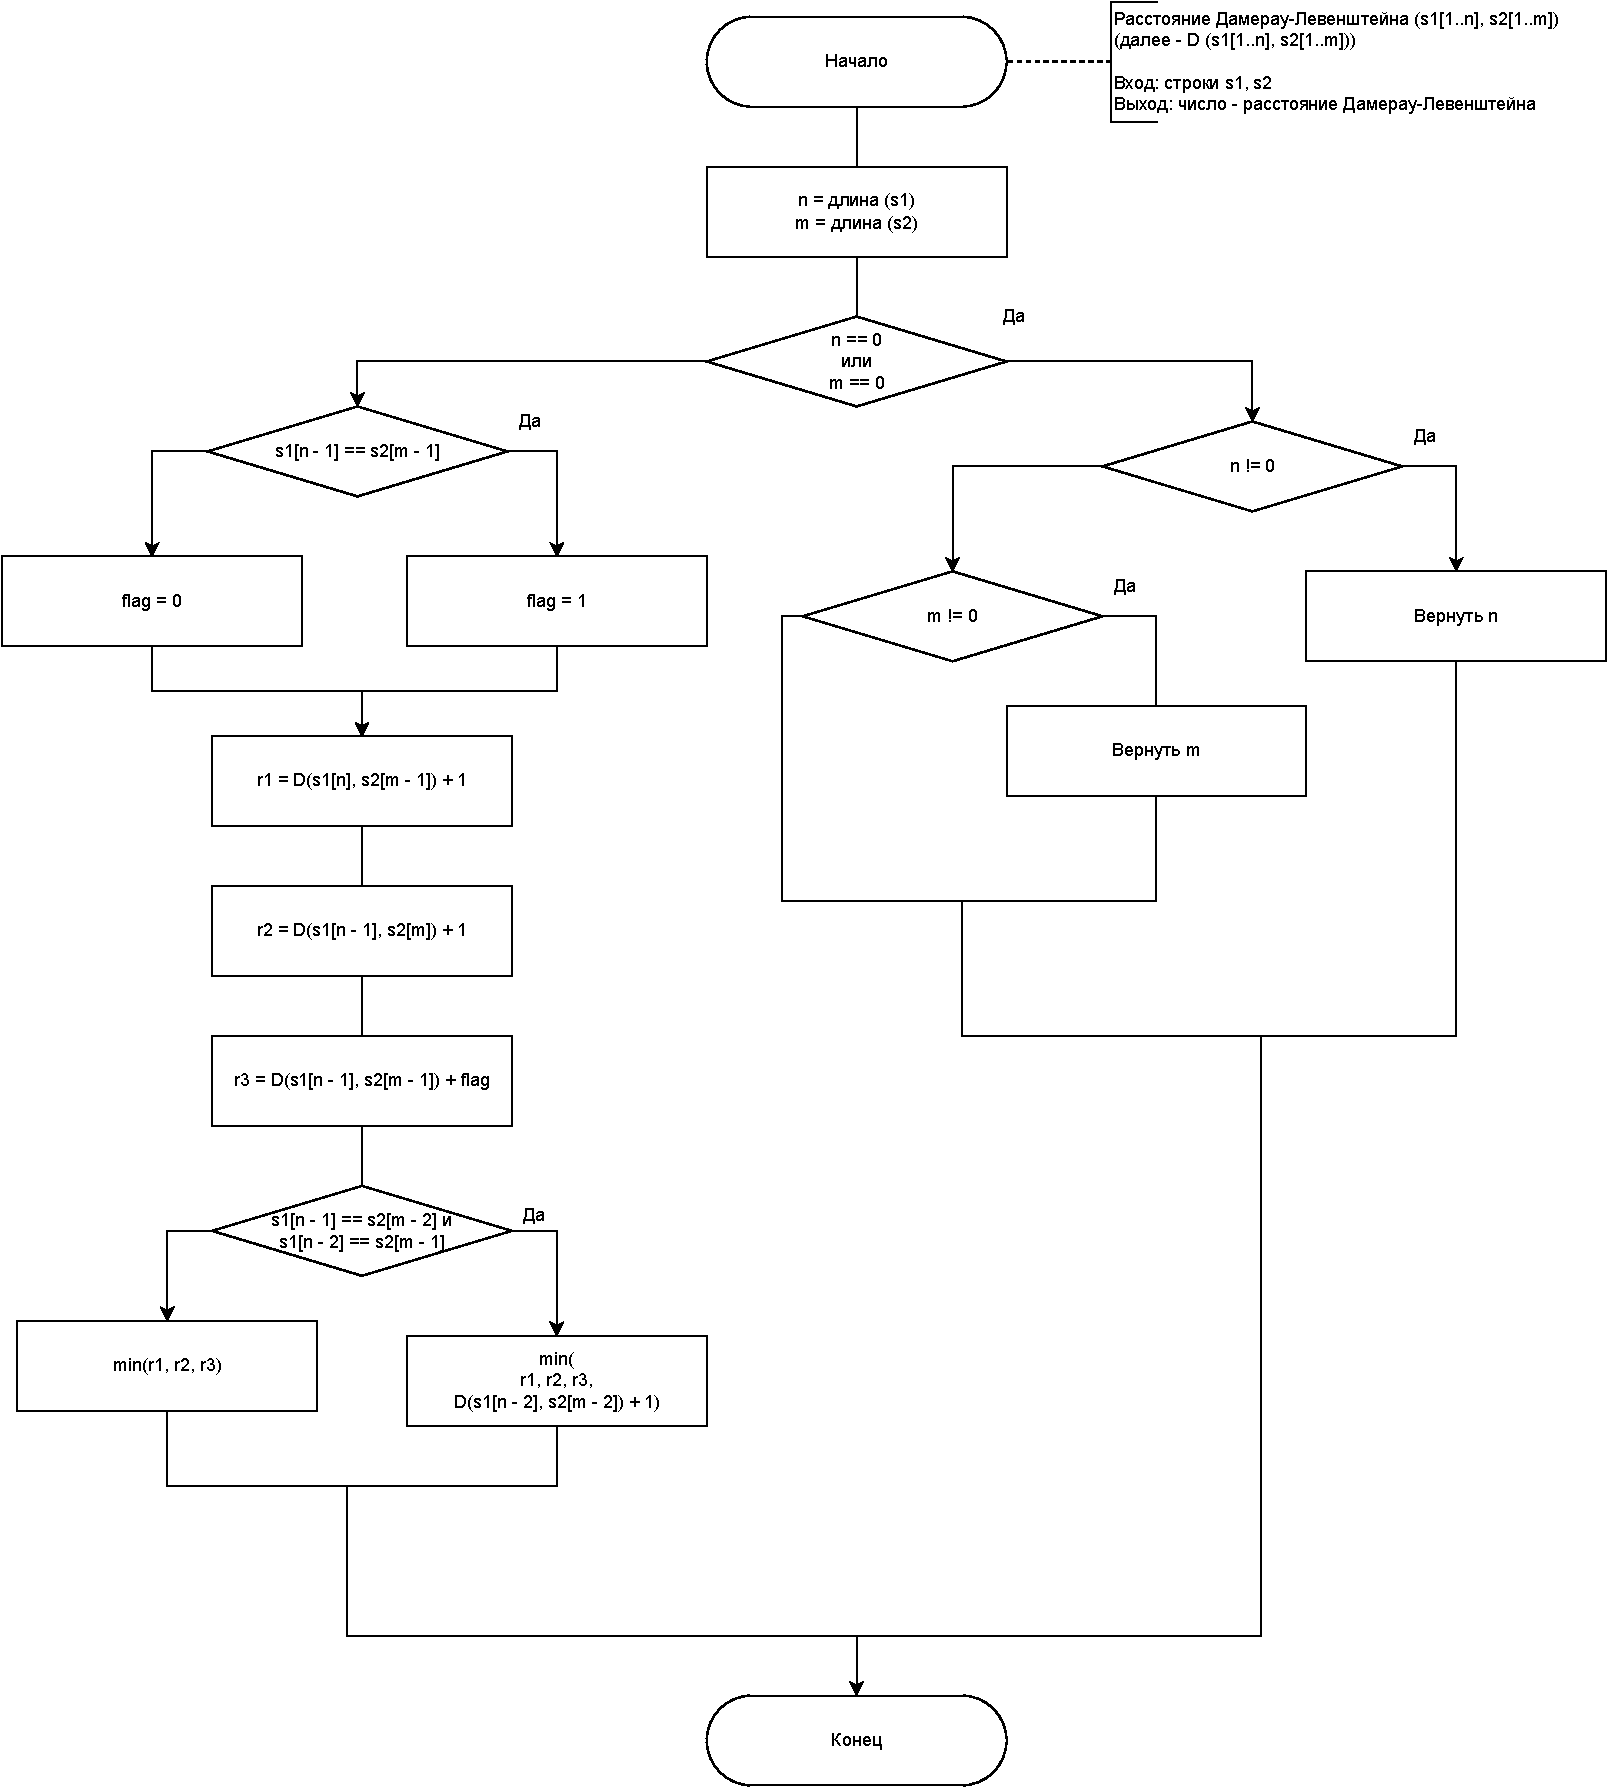
\includegraphics[width=1\linewidth]{include/rec_damlev.pdf}
		\captionof{figure}{Схема рекурсивного алгоритма поиска расстояния \\Дамерау -- Левенштейна}
		\label{img:recdamlev}
	\end{tabular}
\end{table}

Схема рекурсивного с кешированием алгоритма поиска расстояния \\Дамерау -- Левенштейна представлена на рисунке \ref{img:rec_cache_damlev}.

\begin{table}[h!]
	\centering
	\begin{tabular}{p{1\linewidth}}
		\centering
		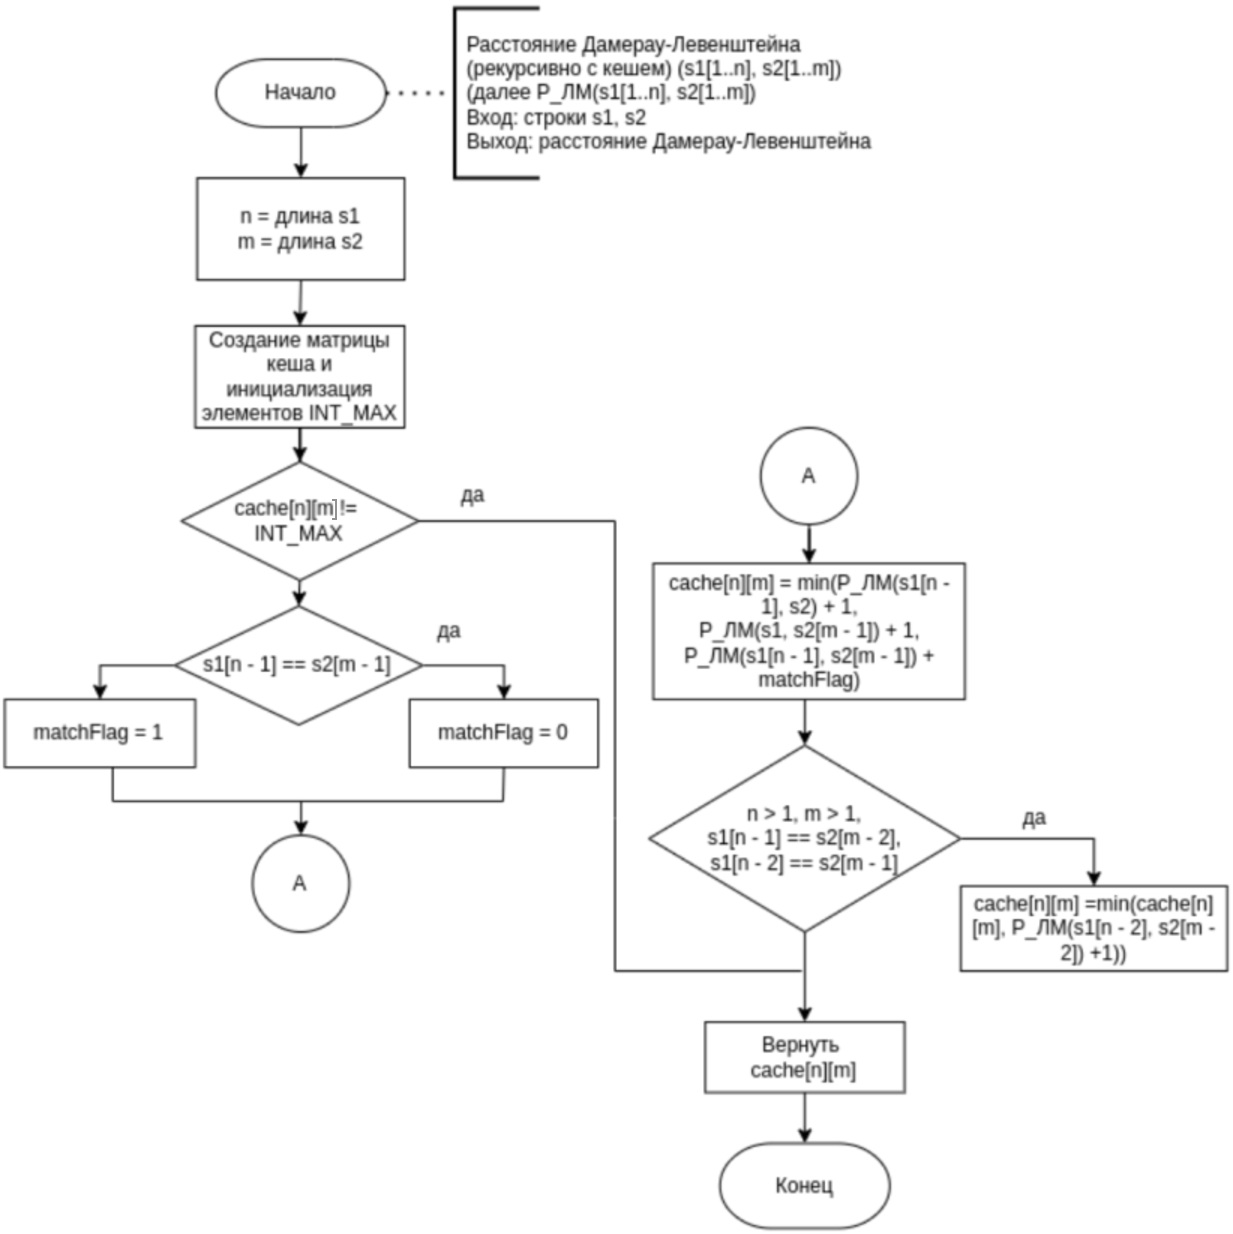
\includegraphics[width=1\linewidth]{include/rec_cache_damlev.pdf}
		\captionof{figure}{Схема рекурсивного с кешированием алгоритма поиска расстояния Дамерау -- Левенштейна}
		\label{img:rec_cache_damlev}
	\end{tabular}
\end{table}
